\chapter{Transmissão de dados em série}\label{chap:chap4}

Este capítulo aborda os processos de serialização e deserialização adotados neste projeto. Estes exigem cuidados e aplicações de determinados métodos que permitam manter a integridade do sinal durante a transmissão do mesmo, como já foi referenciado em \ref{serial_theory}. Foi referido ainda em \ref{sub:arqGTX} que a FPGA VC7203 possui entradas e saídas de alta velocidade com arquiteturas constituídas por blocos que permitem a implementação destes mecanismos. Na figura \ref{fig:gtx_geral_arq} visualiza-se uma arquitetura geral dos transcetores que serão descritos mais detalhadamente daqui em diante.

Este capítulo começa por abordar as arquiteturas transmissora e recetora com detalhe, quais as características que são vantajosas a este projeto e ainda analisa as vantagens e desvantagens de algumas para que se possa fazer a melhor escolha para o projeto. É ainda feita uma análise das características de transmissão e por fim é explicada a estrutura geral do transcetor.

\section{Transmissor} \label{sec:tx_gtx}

Na figura \ref{fig:gtx_tx_arq} visualiza-se a arquitetura do transmissor GTX.  Esta possui blocos com diferentes funções que permitem manter a integridade do sinal durante uma transmissão.

\begin{figure}[h!]
	\begin{center}
		\leavevmode
		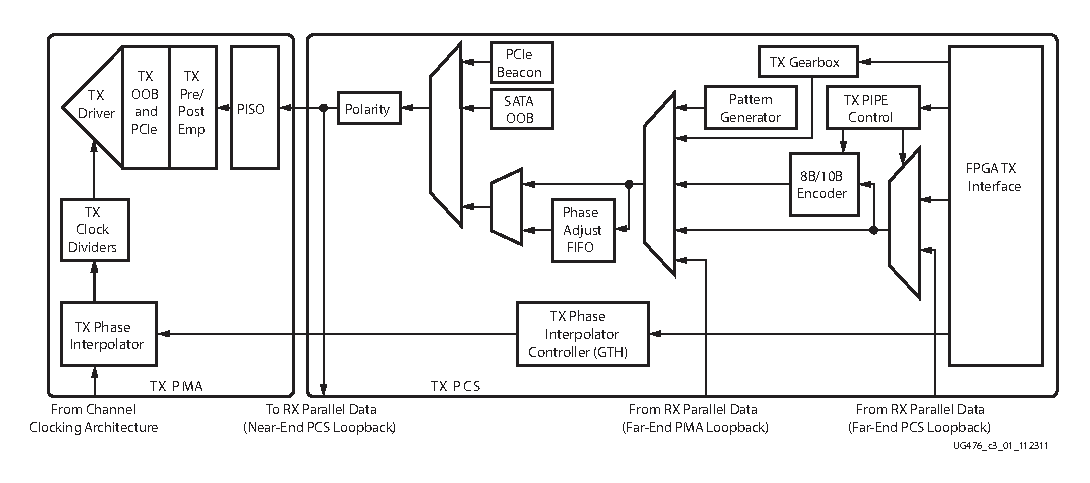
\includegraphics[width=1.0\textwidth]{tx_gtx_arq}
		\caption[Arquitetura do transmissor GTX]{Arquitetura do transmissor GTX (retirada de \cite{R011})}
		\label{fig:gtx_tx_arq}
	\end{center}
\end{figure}

Os blocos mais relevantes para o funcionamento do projeto passam a ser descritos nas próxima subsecções para uma melhor compreensão das arquiteturas desenvolvidas.

\subsection{Interface com a FPGA} \label{subch:tx_interface}

Na figura \ref{fig:gtx_tx_arq} este bloco tem o nome de "\textit{FPGA TX Interface}" sendo a entrada dos dados em paralelo provenientes da FPGA que se pretendem serializar. Segundo \cite{R011}, o tamanho desta interface depende de vários fatores internos. Para se perceber melhor como o tamanho da porta pode variar são apresentados na tabela \ref{table:tx_interface} os casos possíveis.


\begin{table}[h!]
	\centering
		\caption[Tamanhos da interface da FPGA com o GTX transmissor]{Tamanhos da interface da FPGA com o GTX transmissor (adaptada de \cite{R011})}
	\label{table:tx_interface}
	\resizebox{\textwidth}{!}{%
		\begin{tabular}{rlll}
			\hline
			\multicolumn{1}{c}{\textbf{Codificação 8B/10B}} & \multicolumn{1}{c}{\textbf{Tamanho do \textit{datapath}}} & \multicolumn{1}{c}{\textbf{Tamanho Interno}} & \multicolumn{1}{c}{\textbf{Interface com a FPGA}} \\ \hline
			\multicolumn{1}{r|}{Sim}                        & 0 (2 \textit{byte})                                       & 20                                           & 16                                                \\
			\multicolumn{1}{r|}{Sim}                        & 0 (2 \textit{byte})                                       & 20                                           & 32                                                \\
			\multicolumn{1}{r|}{Sim}                        & 1 (4 \textit{byte})                                       & 40                                           & 32                                                \\
			\multicolumn{1}{r|}{Sim}                        & 1 (4 \textit{byte})                                       & 40                                           & 64                                                \\
			\multicolumn{1}{r|}{Não}                        & 0 (2 \textit{byte})                                       & 16                                           & 16                                                \\
			\multicolumn{1}{r|}{Não}                        & 0 (2 \textit{byte})                                       & 20                                           & 20                                                \\
			\multicolumn{1}{r|}{Não}                        & 0 (2 \textit{byte})                                       & 16                                           & 32                                                \\
			\multicolumn{1}{r|}{Não}                        & 1 (4 \textit{byte})                                       & 32                                           & 32                                                \\
			\multicolumn{1}{r|}{Não}                        & 0 (2 \textit{byte})                                       & 20                                           & 40                                                \\
			\multicolumn{1}{r|}{Não}                        & 1 (4 \textit{byte})                                       & 40                                           & 40                                                \\
			\multicolumn{1}{r|}{Não}                        & 1 (4 \textit{byte})                                       & 32                                           & 64                                                \\
			\multicolumn{1}{r|}{Não}                        & 1 (4 \textit{byte})                                       & 40                                           & 80                                                \\ \hline
		\end{tabular}%
	}
\end{table}

Os diferentes tamanhos que a porta da interface pode tomar estão apresentados na última coluna da tabela, tendo em conta que quando é implementada uma codificação, estes apenas podem variar entre 16, 32 ou 64 bits. Todavia, quando não há codificação o tamanho desta porta pode tomar os valores anteriormente referidos ou 20, 40 ou 80 bits. De notar que quando não há codificação e o tamanho da porta é 16, 32 ou 64 bits existe a possibilidade de extender esses valores (caso se pretenda) para 20, 40 e 80 bits respetivamente. No entanto, isto não será abordado dado que não é relevante para o projeto. 

Os valores do tamanho interno do \textit{datapath} podem variar entre 2 e 4 \textit{bytes}. Contudo, convém referir que quando um \textit{datapath} de um determinado tamanho não chega para o número de bits à entrada então é necessário utilizar dois. Este tópico será abordado mais adiante.

%%Relógios que saem e para que servem
Os dados em paralelo entram neste bloco a uma determinada cadência bem definida: ao flanco positivo do sinal de relógio \textit{TXUSRCLK2}, sendo que este é o sinal de sincronização entre os dados provenientes da FPGA com o transmissor. No entanto, é também necessário outro sinal de relógio para a lógica interna PCS do transmissor : \textit{TXUSRCLK}. De recordar que a lógica interna PCS trabalha com os dados em paralelo, portanto o valor deste sinal de relógio depende não só da cadência a que os dados entram no transmissor mas também do \textit{datapath} escolhido. Segundo \cite{R011}, a relação entre estes dois sinais é bem definida e apresentada na tabela \ref{table:freq_tx}.

%Por um lado, o sinal de relógio \textit{TXUSRCLK2} é o principal sinal de sincronização entre a lógica da FPGA e a lógica do transmissor, por outro o sinal de relógio \textit{TXUSRCLK} é a cadência determinista dos dados em paralelo no bloco PCS, e por isso existe uma relação entre estes dois sinais muito bem definida que passa a ser apresentada na tabela na página \pageref{table:freq_tx}.

\begin{table}[h!]
		\caption[Relação das frequências dos sinais de relógio \textit{TXUSRCLK2} e \textit{TXUSRCLK}]{Relação das frequências dos sinais de relógio \textit{TXUSRCLK2} e \textit{TXUSRCLK} (adaptada de \cite{R011})}
	\label{table:freq_tx}
	\centering
	\resizebox{\textwidth}{!}{%
		\begin{tabular}{lll}
			\hline
			\multicolumn{1}{c}{\textbf{Tamanho na Interface}} & \multicolumn{1}{c}{\textbf{Tamanho do \textit{datapath}}} & \multicolumn{1}{c}{\textbf{Relação entre os sinais de relógio}} \\ \hline
			16, 20 (bits)                                     & 0 (2 \textit{byte})                                       & $F_{TXUSRCLK} = F_{TXUSRCLK2}  $                                    \\
			32, 40 (bits)                                     & 0 (2 \textit{byte})                                       & $F_{TXUSRCLK} = F_{TXUSRCLK2} * 2$                                  \\
			32, 40 (bits)                                     & 1 (4 \textit{byte})                                       & $F_{TXUSRCLK} = F_{TXUSRCLK2} $                                      \\
			64, 80 (bits)                                     & 1 (4 \textit{byte})                                       & $F_{TXUSRCLK} = F_{TXUSRCLK2} * 2$                                  \\ \hline
		\end{tabular}%
	}
\end{table}


%Explicar que se pode obter uma estimativa da velocidade de transmissão de acordo com aquela equação
Segundo \cite{R011}, sabendo estas relações entre os sinais de relógio, o tamanho da porta na interface do transmissor e o tamanho do \textit{datapath} usado é possível obter a velocidade de transmissão dos dados em série através da equação apresentada em \ref{eq:lineRate}.

\begin{equation} \label{eq:lineRate}
Line\ Rate = F_{TXUSRCLK}*(Internal\ Datapath\ Width)
\end{equation}


%Explicar pq e que tem frequências diferentes visto que sao os dois para sinais em paralelo
Para que se perceba a diferença entre estas frequências é agora apresentado um caso em concreto que é utilizado neste projeto. Pretende-se na entrada do transmissor obter 40 bits em paralelo e que estes dados sejam amostrados a uma frequência de \SI{148.5}{\mega\hertz} ($F_{TXUSRCLK2} = \SI{148.5}{\mega\hertz}$). Assim sendo, existem agora duas hipóteses: a utilização de um \textit{datapath} de 2 \textit{byte} ou 4 \textit{byte}.

Se se optar pelo \textit{datapath} de 4 \textit{byte} então está-se perante a opção a), ilustrada na figura \ref{fig:exemplo_datapaths} em que o sinal de amostragem à entrada é de \SI{148.5}{\mega\hertz} ($F_{TXUSRCLK2} = \SI{148.5}{\mega\hertz}$) e o sinal de lógica do bloco PCS também é \SI{148.5}{\mega\hertz} ($F_{TXUSRCLK} = \SI{148.5}{\mega\hertz}$). Neste caso a largura do sinal interno é de 40 bits o que, segundo a equação \ref{eq:lineRate}, perfaz uma taxa de saída dos dados em série de \SI{5.94}{\giga\bit\per\second}.

Por outro lado, se se optar por um \textit{datapath} interno de 2 \textit{byte} serão necessários 2 \textit{datapath}, com largura interna de 20 bits cada, tal como ilustra o caso b) da figura \ref{fig:exemplo_datapaths}. Isto implica que a taxa de amostragem nesses seja o dobro da cadência de entrada dos sinais na interface com transmissor. Assim, mantém-se uma frequência de amostragem à entrada do transmissor de $F_{TXUSRCLK2} = \SI{148.5}{\mega\hertz}$ e uma frequência do sinal de relógio de cada bloco PCS de $F_{TXUSRCLK} = \SI{297}{\mega\hertz} $. Segundo a equação \ref{eq:lineRate}, a taxa de débito de saída é \SI{5.94}{\giga\bit\per\second}.

\begin{figure}[h!]
 	\begin{center}
 		\leavevmode
 		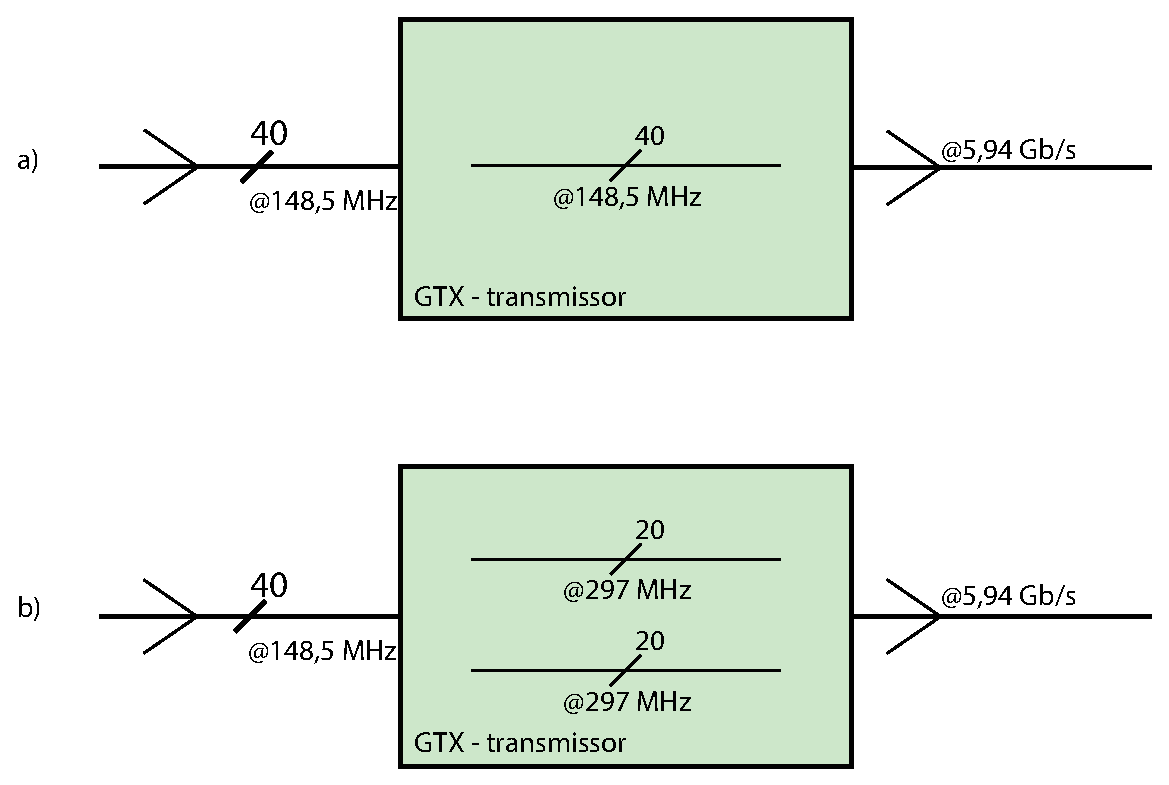
\includegraphics[width=0.75\textwidth]{exemplo_datapath}
 		\caption[Exemplo simplificado de transmissão com diferentes usos de \textit{datapath}]{Exemplo simplificado de transmissão com diferentes usos de \textit{datapath}}
 		\label{fig:exemplo_datapaths}
 	\end{center}
 \end{figure}

%%Concluir como se geram estes sinais
Estes dois sinais de relógio, gerados neste bloco, são colocados nas saídas do mesmo para que na FPGA possa ser desenvolvida uma arquitetura que leia os sinais em paralelo para o transmissor à cadência de \textit{TXUSRCLK2}. Estes estão alinhados pelo flanco positivo de ambos ainda que tenham frequências diferentes. De notar ainda que os mesmo são gerados com base no sinal de relógio de referência, segundo \cite{R011} e \cite{R022}, através de multiplicadores ou divisores caso possuam frequências diferentes.


\subsection{Codificador 8B/10B}

Este bloco, quando ativo, permite que os sinais em paralelo sejam codificados de 8 para 10 bits. É de notar que, apesar de ser vantajosa a utilização de codificação num protocolo de transmissão em série, a ativação deste bloco aumenta a latência do transmissor.

As características deste tipo de codificação, as suas vantagens e importância foram já abordadas na subsecção \ref{subsub:cod_impor} na página \pageref{subsub:cod_impor}.


\subsection{Interface entre os diferentes domínios de sinal de relógio do transmissor} \label{subsub:tx_buffer}

Já foi referido anteriormente que para o correto funcionamento o transmissor GTX opera com pelo menos dois sinais de relógio diferentes : TXUSRCLK and TXUSRCLK2. O segundo é o sinal de relógio de sincronização principal entre os dados provenientes da FPGA e o transmissor, e o primeiro é o sinal de relógio utilizado para a lógica do bloco PCS.

Contudo, o bloco PCS utiliza dois sinais de relógio internamente para o seu correto funcionamento: TXUSRCLK (como já foi mencionado) e ainda XCLK (sinal de relógio dos dados em paralelo do bloco PMA). A figura \ref{fig:clk_domains_tx} ilustra os diferentes domínios de relógio presentes no transmissor GTX.

\begin{figure}[h!]
	\begin{center}
		\leavevmode
		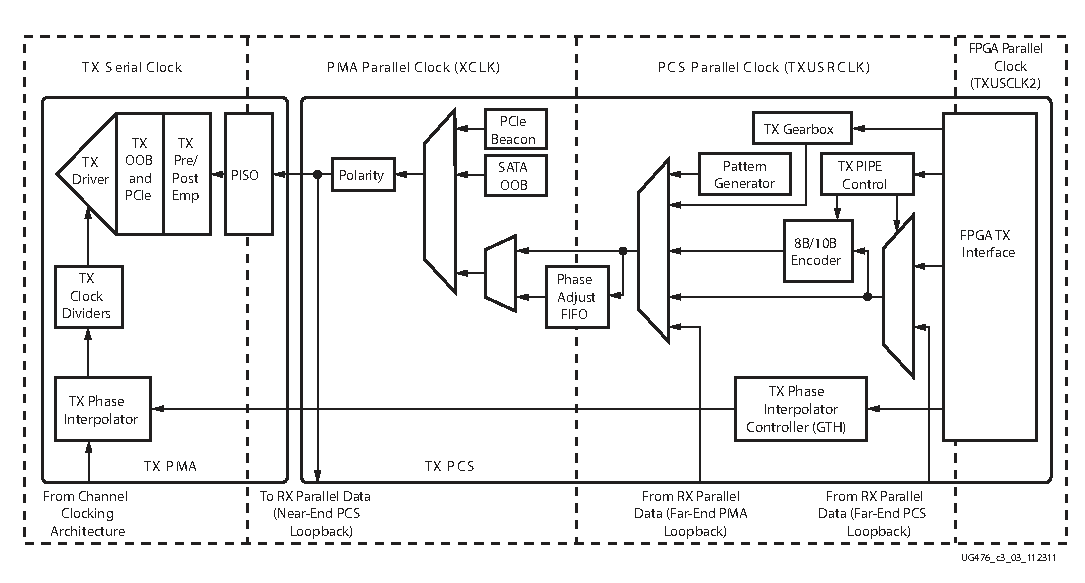
\includegraphics[width=1.0\textwidth]{clk_domain_cross_gtx_tx}
		\caption[Diferentes domínios de sinal de relógio do transmissor]{Diferentes domínios de sinal de relógio do transmissor (retirada de \cite{R011})}
		\label{fig:clk_domains_tx}
	\end{center}
\end{figure}

Quando os dados são transferidos entre os domínios TXUSRCLK e XCLK é necessário que para além de terem frequências semelhantes, as diferenças de fase que possam existir estejam resolvidas. Por isso, existem dois blocos responsáveis por tal que apresentam os seus prós e contras: \textit{buffer} ou bloco de alinhamento de fase. Independentemente da escolha de um ou de outro, a utilização de um deles é obrigatória e torna-se importante conhecer as suas vantagens e desvantagens, pois tal escolha afeta o funcionamento global do sistema, segundo \cite{R011}.

Por um lado, a utilização de um \textit{buffer} é mais fácil e ainda assim é robusta, enquanto que o bloco de alinhamento de fase exige a utilização de mais lógica e restrições de sinais de relógio adicionais. Por outro lado, quando a latência se torna um ponto importante do sistema, a utilização do \textit{buffer} deve ser posta de lado, visto que o bloco de alinhamento de fase utiliza menos registos obtendo assim uma latência menor.

\subsection{Interface com a camada física} 
Após a serialização dos dados no bloco PISO da figura \ref{fig:gtx_tx_arq} os sinais são transmitidos para a camada física através de um \textit{driver} reconfigurável. Esta interface dispões de várias características que permitem manter a integridade do sinal que passam de seguida a ser apresentadas:

\begin{itemize}
	\item \textbf{Sinalização Diferencial:} para diminuir eventuais interferências no sinal durante a sua transmissão no cabo físico, tal como mencionado na subsecção  \ref{subsub:sinalizacao_fisica} na página \pageref{subsub:sinalizacao_fisica}.
	
	\item \textbf{Pré-ênfase:} para preparar o sinal para um canal ruidoso, tal como referido na subsecção \ref{subsub:pre_enfase_equalizacao} na página \pageref{subsub:pre_enfase_equalizacao}.
	
	\item \textbf{Resistências de interface com o cabo calibráveis:} para que a impedância característica da linha esteja adaptada com a interface evitando assim eventuais reflexões dos sinais, tal como mencionado na subsecção \ref{subsub:restricoes_circuitos} na página \pageref{subsub:restricoes_circuitos}.
\end{itemize}


\section{Recetor} \label{sec:_rx_gtx}
Na figura \ref{fig:gtx_rx_arq} é possível visualizar a arquitetura do recetor GTX. Este inclui diversos blocos que permitem a correta recuperação do sinal, sendo que o funcionamento dos principais já foi mencionado na subsecção \ref{serial_theory}. Assim, passa-se de seguida à descrição dos mesmos.

\begin{figure}[h!]
	\begin{center}
		\leavevmode
		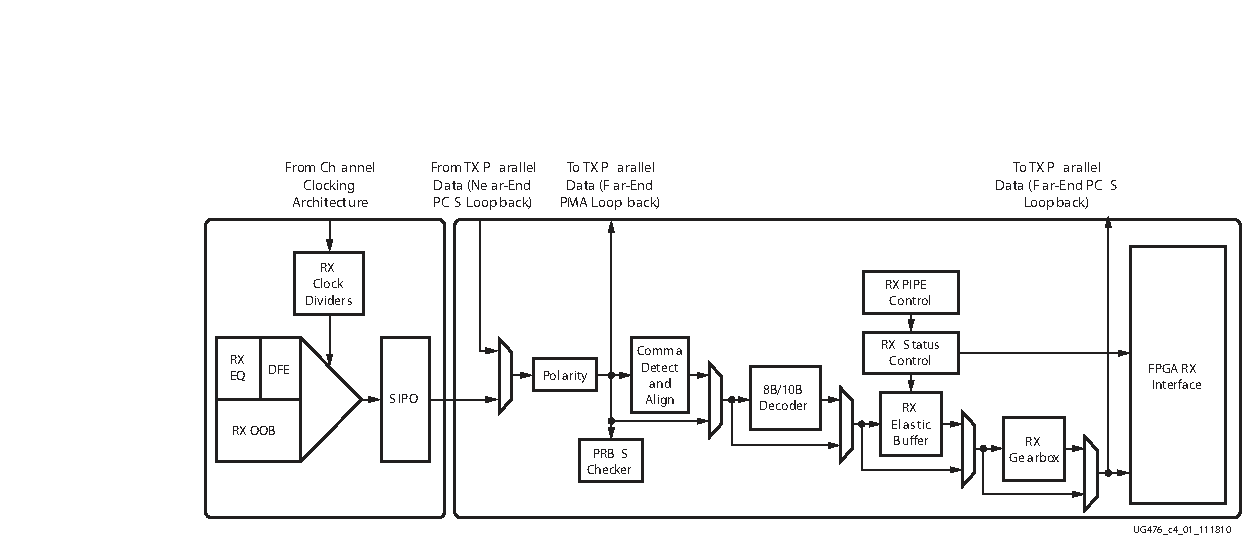
\includegraphics[width=1.0\textwidth]{rx_gtx_arq}
		\centering
		\caption[Arquitetura do recetor GTX]{Arquitetura do recetor GTX, (retirada de \cite{R011})}
		\label{fig:gtx_rx_arq}
	\end{center}
\end{figure}
	

\subsection{Interface com a camada física}

A interface o cabo físico do recetor possui duas características importantes para a recuperação do sinal:
\begin{itemize}
	\item \textbf{Tensão de terminação configurável:} Esta característica é importante quando a referência do sinal diferencial é variável do lado do transmissor o que permite recuperar corretamente o sinal diferencial do lado do recetor.
	
	\item \textbf{Resistências de interface com o cabo configuráveis:} tal como acontecia do lado do transmissor, esta característica torna-se importante para que a linha de transmissão esteja adaptada ao recetor evitando assim eventuais reflexões do sinal.
\end{itemize}


\subsection{Equalização} \label{subsub:rx_equalização}

Na subsecção \ref{subsub:pre_enfase_equalizacao} na página \pageref{subsub:pre_enfase_equalizacao} foi abordada a importância da utilização de filtros equalizadores para tentar compensar a atenuação e distorção que o sinal sofre durante a transmissão no canal físico. O recetor GTX disponibiliza dois tipos de equalizadores adaptativos que devem ser escolhidos consoante as necessidades de consumo de potência do circuito \textit{versus} perdas do canal físico de transmissão.

Segundo \cite{R011}, para canais cujas perdas não são muito significativas e o consumo de potência torna-se uma característica crítica do circuito existe um filtro adaptativo otimizado com o nome de LPM (\textit{Low-power mode}). Ainda segundo esta fonte, o uso deste tipo de equalizador é recomendado para aplicações com débitos até \SI{11.2}{\giga\bit\per\second} de curto alcance e com perdas por canal até \SI{12}{\decibel} à frequência de \textit{Nyquist}.


Para canais cujas perdas se tornam significativas existe disponível um filtro adaptativo com o nome de \textit{Decision Feedback Equalizer} (DFE). 
%Este é um filtro que utiliza a realimentação de símbolos detetados para produzir uma estimação da saída do canal. 
Segundo \cite{R011}, este equalizador é utilizado para ligações de média distância cujas perdas do canal rondam os \SI{8}{\decibel} ou mais à frequência de \textit{Nyquist}. Este equalizador apresenta ainda as seguintes vantagens:
\begin{itemize}
	\item Efetua a equalização sem amplificação do ruído ou eventuais interferências;
	\item Pode também fazer correções de reflexões causadas pelas descontinuidades do canal.
\end{itemize}

%\textbf{Cuidados a ter na utilização deste tipo de equalizador:}
%\begin{itemize}
%	\item Este tipo de equalização deve ser cuidadosa quando não existe codificação de dados, uma vez que pode levar à não equalização ideal do sinal recebido (pois o filtro pode não se auto adaptar aos dados recebidos).
%\end{itemize}

Tendo em conta as vantagens dos dois equalizadores disponíveis no recetor GTX, verifica-se que a utilização de cada um deles pode ser utilizada em circunstâncias diferentes. Numa fase inicial pode ser utilizado um equalizador DFE, apesar de gastar mais energia, contudo a utilização de um equalizador LPM reduz o consumo. Numa fase mais avançada do projeto, que envolva a inserção dos sinais em ligações longas e/ou ruidosas, faz mais sentido usar um filtro DFE adaptado para tal. 



%
%Conhecendo agora os prós e contras dos dois equalizadores disponíveis no recetor GTX conclui-se que numa fase inicial do projeto em que nao se pretende usar codificação, e uma ligação curta não faz sentido usar um equalizador DFE, mas sim um equalizador LPM. T

%\subsection{CDR - \textit{Clock And Data Recovery}}
%
%No recetor GTX, existe um bloco responsável por uma característica muito importante de um transcetor: recuperação de sinal de relógio e dados. Segundo \cite{R011}, esse circuito faz a recuperação do relógio e dos dados através do \textit{stream} de dados que recebe. A figura \ref{fig:cdr_arq} da página \pageref{fig:cdr_arq} ilustra esse mesmo bloco.
%
%\begin{figure}[h!]
%	\begin{center}
%		\leavevmode
%		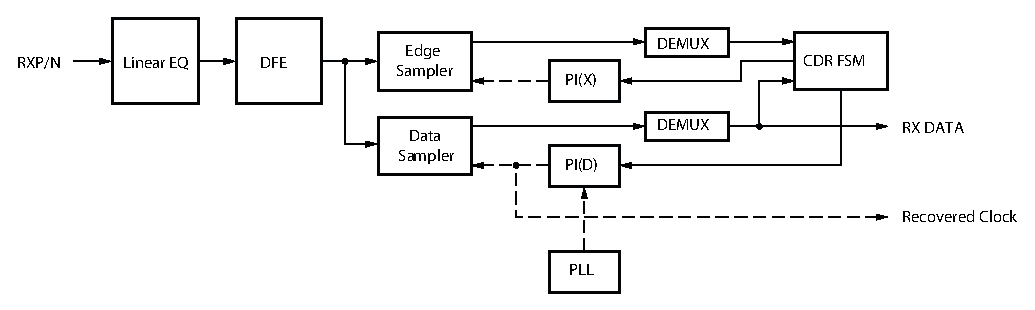
\includegraphics[width=1.0\textwidth]{cdr_arq_vet}
%		\caption{Arquitetura do circuito de recuperação de sinal de relógio e dados, retirada de \cite{R011}}
%		\label{fig:cdr_arq}
%	\end{center}
%\end{figure}
%
%%Os dados recebidos passam pelo equalizador e de seguida são capturados por um “\textit{data sampler}” e um “\textit{edge sampler}”. O “\textit{edge sampler}” captura a fase do sinal recebido em série quando este está na sua região de transição, enquanto que o “\textit{data sampler}” captura a fase do mesmo sinal a meio do olho dos dados, tal como ilustra a figura \ref{fig:exmple_cdr} da página \pageref{fig:exmple_cdr}.  Estas duas fases são de seguida enviadas para a máquina de estados do CDR para que esta consiga determinar a fase dos sinais que chegam e ao mesmo tempo controlar os interpoladores de fase (PIs). 
%
%
%\begin{figure}[h!]
%	\begin{center}
%		\leavevmode
%		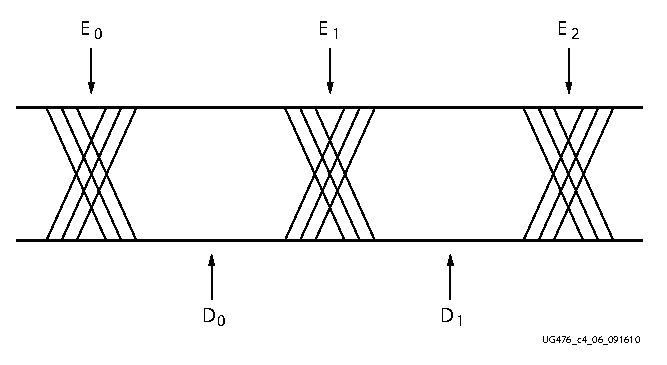
\includegraphics[width=0.5\textwidth]{exemplo_cdr}
%		\captionsetup{width=0.5\linewidth}
%		\caption{Exemplo das amostras de fase retiradas do circuito, retirada de \cite{R011}}
%		\label{fig:exmple_cdr}
%	\end{center}
%\end{figure}
%
%Na figura \ref{fig:exmple_cdr} E0, E1 e E2 correspondem ás amostras retiradas pelo "\textit{edge sampler}" e D0 e D1 às amostras retiradas pelo "\textit{data sampler}".
%A tracejado na figura \ref{fig:cdr_arq} visualiza-se o sinal de relógio recuperado com o nome de "\textit{Recovered Clock}" e os dados recuperados em série saem no sinal "\textit{RXDATA}".


\subsection{Alinhamento de Palavras} \label{subsub:align}

O bloco de alinhamento de palavras é feito antes da deserialização dos dados, isto porque é necessário definir os limites das palavras antes destes serem convertidos para o formato em paralelo. O método de alinhamento de palavras, os símbolos especiais existentes para aplicação neste método e ainda a sua importância foram já abordados na subsecção \ref{subsub:alinhamento} na página \pageref{subsub:alinhamento}.

Nesta subsecção serão abordadas as características que este bloco do recetor possui e ainda como se pode tirar partido das mesmas aquando da sua utilização. O bloco possibilita a escolha da palavra de alinhamento que se pretende utilizar, sendo que se pode tirar partido de um protocolo já conhecido para a escolha desta.

Apesar de existirem \textit{flags}\footnote{uma \textit{flag} é uma variável de controlo binária para identificar determinadas condições} disponibilizadas pelo bloco de alinhamento que indicam o estado do mesmo, o autor de \cite{R011} alerta que para uma linha de transmissão cuja taxa de débito é superior a \SI{5}{\giga\bit\per\second}, o bloco pode alinhar a palavra falsamente ativando \textit{flag} que indica que a palavra está alinhada, mesmo não estando. Isto implica que seja desenvolvido e aplicado um sistema que verifique se a palavra se encontra devidamente alinhada ou não.

%%Alinhamento Manual

Este bloco dispõe de uma opção de alinhamento manual que vem substituir o automático, o que pode ser bastante útil em casos onde o transcetor alinha falsamente uma palavra. Na figura \ref{fig:rxslide_example} é possível visualizar o exemplo de alinhamento manual das palavras no recetor que passa a ser descrito.

\begin{figure}[h!]
	\begin{center}
		\leavevmode
		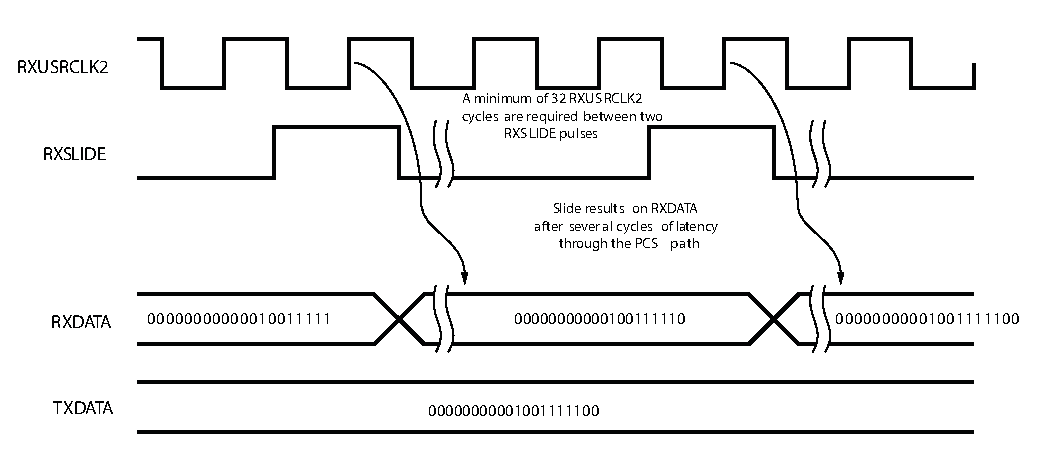
\includegraphics[width=1.0\textwidth]{rxslide_example}
		\captionsetup{width=1.0\linewidth}
		\caption[Exemplo de um alinhamento manual da palavra]{Exemplo de um alinhamento manual da palavra (retirada de \cite{R011})}
		\label{fig:rxslide_example}
	\end{center}
\end{figure}

Este processo de alinhamento manual é conhecido pelo nome de "\textit{RXSLIDE}" e é usado para mover a palavra em 1 bit. Este sinal deve estar ativo apenas um ciclo de relógio de RXUSRCLK2 e de seguida deve ser inativo. Segundo \cite{R011}, deve-se esperar pelo menos 32 ciclos de relógio para que esta operação seja realizada outra vez. Este tempo de espera relaciona-se com o tamanho do \textit{datapath} usado.

\subsection{Descodificador 8B/10B}

Tal como no transmissor, este bloco é responsável pela descodificação 8B/10B caso esta tenha sido ativada do lado do transmissor. Esta operação é realizada depois da conversão dos dados para paralelo e é de notar que a utilização deste bloco aumenta a latência de todo o sistema.

Numa fase inicial do projeto, a utilização deste bloco (tanto do lado do transmissor como do recetor) é posta de lado no sentido de simplificar o mesmo e também de diminuir a latência do sistema.   

\subsection{Interfaces entre os diferentes domínios de sinal relógio do recetor} \label{subsub:rx_buffer}

Tal como acontecia no transmissor, o recetor opera a diferentes domínios de sinal de relógio. Particularmente no bloco PCS existem dois domínios de relógio para os dados em paralelo críticos: RXUSRCLK e XCLK(o sinal de relógio dos dados em paralelo do bloco PMA). A figura \ref{fig:dominios_rx} ilustra os diferentes domínios de relógio presentes no recetor.

\begin{figure}[h!]
	\begin{center}
		\leavevmode
		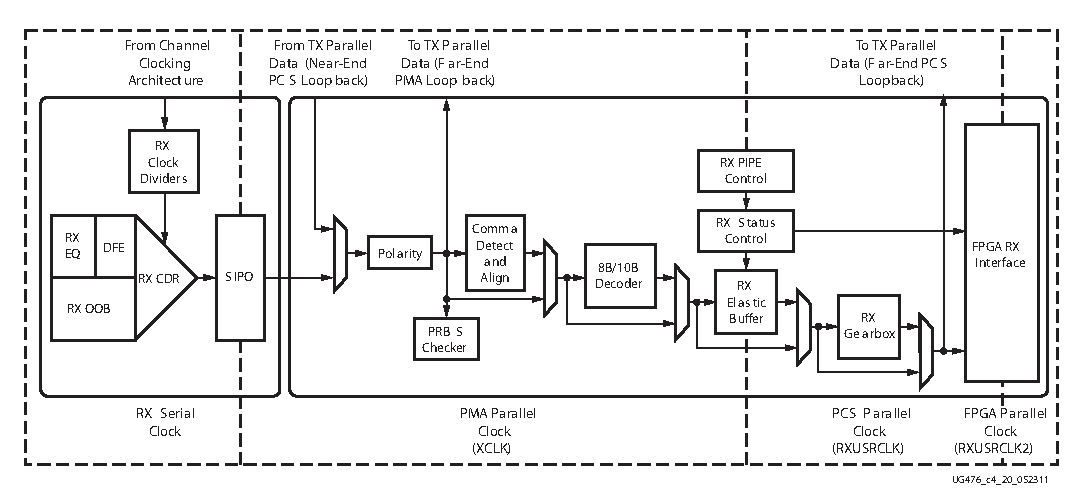
\includegraphics[width=1.0\textwidth]{dominios_rx}
		\captionsetup{width=1.0\linewidth}
		\caption[Diferentes domínios de sinal de relógio no recetor]{Diferentes domínios de sinal de relógio no recetor (retirada de \cite{R011})}
		\label{fig:dominios_rx}
	\end{center}
\end{figure}

Quando os dados são transmitidos de um domínio para o outro todas as diferenças de fase entre os sinais de relógio devem estar resolvidas e a frequência não deve variar muito. Por este motivo deve usar-se um dos dois seguintes blocos: \textit{elastic buffer} ou bloco de alinhamento de fase. Ambos os blocos resolvem as diferenças de fase entre os dois domínios, no entanto apresentam as suas vantagens e desvantagens.

Se por um lado, segundo \cite{R011}, o \textit{buffer} é uma estrutura robusta e de fácil operação, enquanto que o bloco de alinhamento de fase exige mais lógica e restrições relativamente às fontes de relógio. Por outro lado, o uso do \textit{buffer} implica uma latência maior visto que o bloco de alinhamento de fase foi concebido para diminuir a latência total do sistema. 

O \textit{buffer} tem a capacidade de se inicializar imediatamente, enquanto que o circuito de alinhamento de fase tem de esperar que todos os sinais de relógio estabilizem para poder conseguir operar corretamente. Quanto à correção do sinal de relógio, o uso do\textit{ elastic buffer} é obrigatório, enquanto que a utilização do bloco de alinhamento de palavras exige que esta correção seja feita fora do transcetor.

Assim sendo, o uso do bloco de alinhamento torna-se útil quando a latência é um requisito crítico do sistema, todavia o uso do \textit{buffer} não requer correção de sinal de relógio externa ao transcetor o que simplifica bastante o sistema. É uma boa opção numa fase inicial do projeto utilizar um \textit{buffer} para fazer as correções de fase, pois, apesar de introduzir um pouco de latência no circuito, não exige lógica externa ao transcetor para correção do sinal de relógio.

\subsection{Interface com a FPGA}

Este é o bloco responsável pela conexão entre os dados do recetor com o resto da FPGA. Toda a lógica desenvolvida na FPGA deve receber os dados provenientes do recetor pela porta "RXDATA" lendo-os ao flanco positivo do sinal de relógio "RXUSRCLK2". O tamanho desta porta depende de vários fatores internos do recetor, tal como acontecia no transmissor,  como por exemplo se a codificação está ativa ou não e ainda qual o tamanho do \textit{datapath} usado (2 ou 4 \textit{byte}). As diferentes possibilidades de largura da porta de "RXDATA" assemelham-se às da largura da porta de entrada do transmissor (TXDATA), e por isso é possível encontrá-las na tabela \ref{table:tx_interface}.

Também à semelhança do transmissor existem dois sinais de relógio necessários para o correto funcionamento do recetor: RXUSRCLK e RXUSRCLK2. O segundo já foi mencionado como o sinal de relógio de sincronização entre o recetor e a lógica da FPGA, e o sinal de relógio RXUSRCLK é o sinal interno para a lógica do bloco PCS (que lida com os dados em paralelo). O valor deste relógio depende da velocidade de transmissão do canal e do tamanho interno do \textit{datapath} usados, sendo possível calcular o seu valor através da equação presente em \ref{eq:lineRate}.

A relação entre estes dois sinais de relógio mencionados (RXUSRCLK e RXUSRCLK2) é bem definida, dependendo do tamanho da porta "RXDATA" e do tamanho do \textit{datapath} usado.  A relação entre estes dois sinais de relógio do recetor é idêntica à do transmissor e por isso é possível encontrar essas mesmas relações na tabela \ref{table:freq_tx}.

\section{Análise das características de transmissão}

Nesta secção são abordadas as diferentes características de transmissão possíveis de obter (velocidades de transmissão, tamanho de tramas entre outras) tendo em conta as restrições dos GTX, de maneira a otimizar a transmissão.

O projeto pode ser abordado de várias maneiras, desde a restrição da largura de banda base da transmissão até à limitação do número de bits por tramas. No sentido de simplificar o projeto e torná-lo eficiente em termos lógicos restringiu-se a cadência de entrada dos dados no transcetor para \SI{148.5}{\mega\hertz}. Deste modo, não é necessário o uso de memórias, por exemplo FIFO, para armazenar dados antes da sua entrada nos transcetores.

Com esta restrição, e para se retirar algumas conclusões relativamente à otimização de transmissão dos dados em série, efetuaram-se cálculos de débitos de transmissão para as diferentes larguras na porta de dados. Para efetuar estes cálculos utilizou-se a equação apresentada em \ref{eq:lineRate}. Esses resultados estão apresentados na tabela \ref{table:line_rates}.

\begin{table}[h!]
	\centering
	\caption[Débitos de transmissão para diferentes larguras de porta de entrada do transcetor]{Débitos de transmissão para diferentes larguras de porta de entrada do transcetor}
	\label{table:line_rates}
	\resizebox{\textwidth}{!}{%
		\begin{tabular}{@{}lllllll@{}}
			\toprule
			\textbf{\begin{tabular}[c]{@{}l@{}}Interface\\ com a \\ FPGA\end{tabular}} & \textbf{\begin{tabular}[c]{@{}l@{}}Codificação \\ 8B/10B\end{tabular}} & \textbf{\begin{tabular}[c]{@{}l@{}}Tamanho \\ do \textit{Datapath}\end{tabular}} & \textbf{\begin{tabular}[c]{@{}l@{}}Tamanho \\ interno \\ do \textit{datapath}\end{tabular}} & \textbf{$F_{TXUSRCLK} $} & \textbf{$F_{TXUSRCLK2}$} & \textbf{\begin{tabular}[c]{@{}l@{}}Velocidade \\ em série\end{tabular}} \\ \toprule
			\multirow{2}{*}{16}                                                        & Sim                                                                    & 2 \textit{byte}                                                                  & 20                                                                                 & \SI{148.5}{\mega\hertz}             & \SI{148.5}{\mega\hertz}              & \SI{2.97}{\giga\bit\per\second}                                                               \\
			& Não                                                                    & 2 \textit{byte}                                                                  & 16                                                                                 & \SI{148.5}{\mega\hertz}             & \SI{148.5}{\mega\hertz}               & \SI{2.376}{\giga\bit\per\second}                                                              \\ \hline
			20                                                                         & Não                                                                    & 2 \textit{byte}                                                                  & 20                                                                                 & \SI{148.5}{\mega\hertz}              & \SI{148.5}{\mega\hertz}               & \SI{2.97}{\giga\bit\per\second}                                                               \\ \hline
			\multirow{4}{*}{32}                                                        & Sim                                                                    & 2 \textit{byte}                                                                  & 20                                                                                 & \SI{297}{\mega\hertz}                & \SI{148.5}{\mega\hertz}               & \SI{5.94}{\giga\bit\per\second}                                                              \\
			& Não                                                                    & 2 \textit{byte}                                                                  & 16                                                                                 & \SI{297}{\mega\hertz}                & \SI{148.5}{\mega\hertz}               & \SI{4,752}{\giga\bit\per\second}                                                              \\
			& Sim                                                                    & 4 \textit{byte}                                                                  & 40                                                                                 & \SI{148.5}{\mega\hertz}             & \SI{148.5}{\mega\hertz}               & \SI{5.94}{\giga\bit\per\second}                                                               \\
			& Não                                                                    & 4 \textit{byte}                                                                  & 32                                                                                 & \SI{148.5}{\mega\hertz}              & \SI{148.5}{\mega\hertz}               & \SI{4.752}{\giga\bit\per\second}                                                              \\ \hline
			\multirow{2}{*}{40}                                                        & Não                                                                    & 2 \textit{byte}                                                                  & 20                                                                                 & \SI{297}{\mega\hertz}                & \SI{148.5}{\mega\hertz}               & \SI{5.94}{\giga\bit\per\second}                                                               \\
			& Não                                                                    & 4 \textit{byte}                                                                  & 40                                                                                 & \SI{148.5}{\mega\hertz}             & \SI{148.5}{\mega\hertz}               & \SI{5.94}{\giga\bit\per\second}                                                               \\ \hline
			\multirow{2}{*}{64}                                                        & Sim                                                                    & 4 \textit{byte}                                                                  & 40                                                                                 & \SI{297}{\mega\hertz}                & \SI{148.5}{\mega\hertz}              & \SI{11.88}{\giga\bit\per\second}                                                              \\
			& Não                                                                    & 4 \textit{byte}                                                                  & 32                                                                                 & \SI{297}{\mega\hertz}z                & \SI{148.5}{\mega\hertz}               & \SI{9.5}{\giga\bit\per\second}                                                                \\ \hline
			80                                                                         & Não                                                                    & 4 \textit{byte}                                                                  & 40                                                                                 & \SI{297}{\mega\hertz}                & \SI{148.5}{\mega\hertz}               & \SI{11.8}{\giga\bit\per\second}                                                              \\ \toprule
		\end{tabular}%
	}
\end{table}


Pela tabela \ref{table:line_rates}, verifica-se que, fixando a taxa de amostragem do sinal à entrada do transmissor, é possível obter diversas taxas de transmissão para diferentes larguras da porta de interface com a FPGA. O projeto pode utilizar diferentes larguras de tramas a transmitir, consoante a transmissão que é realizada: uma transmissão apenas de imagem não necessita de transmitir tantos dados como uma transmissão de imagem e som, obtendo-se assim diferentes débitos de linha.

A escolha da largura das tramas a ser transmitido bem como a motivação para tal são abordados aquando da apresentação de cada arquitetura transmitida.

\section{Estrutura do transcetor GTX}

Esta secção apresenta a estrutura geral do IP disponibilizado pela \textit{Xilinx} gerado no \textit{software} VIVADO, mais concretamente todas as suas entradas e saídas no sentido de se poder perceber as características do mesmo.  Para gerar este módulo existe uma interface do \textit{software} VIVADO que permite configurar as diversas características do transmissor e do recetor GTX apresentadas nas secções \ref{sec:tx_gtx} e \ref{sec:_rx_gtx} respetivamente. 

\begin{figure}[h!]
	\begin{center}
		\leavevmode
		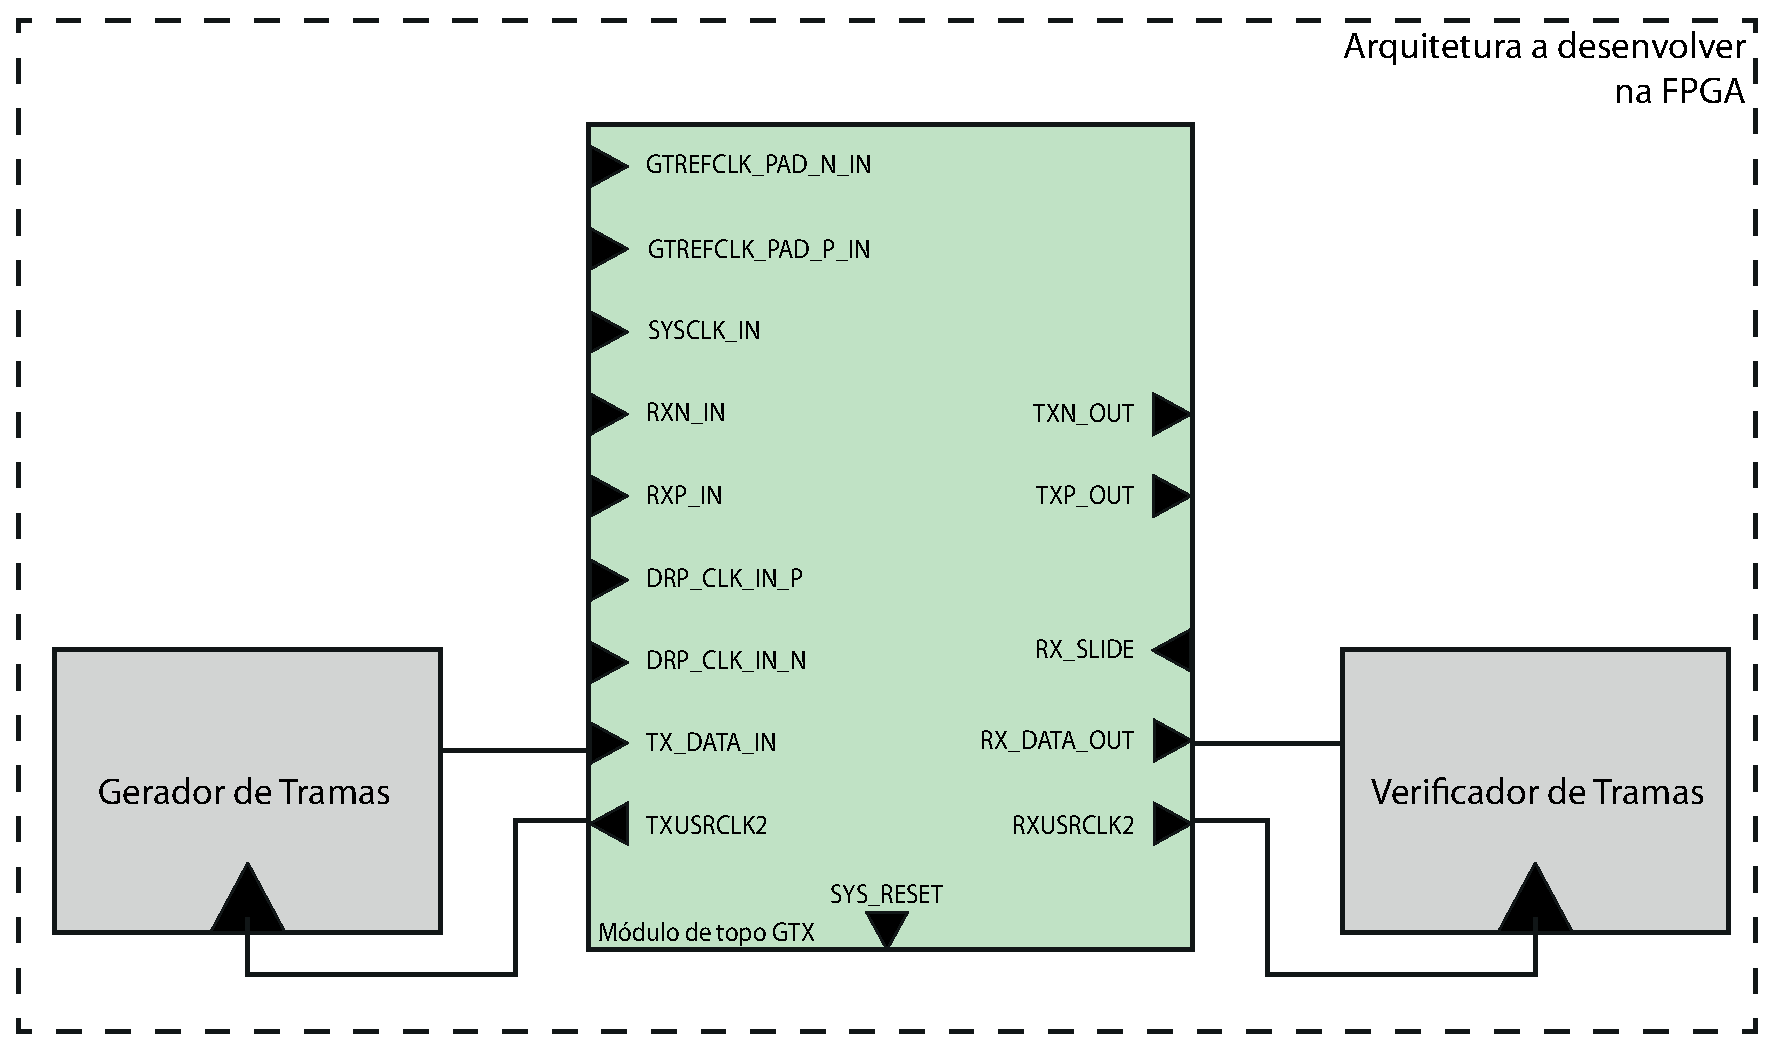
\includegraphics[width=1.0\textwidth]{gtx_wrapper}
		\captionsetup{width=1.0\linewidth}
		\caption[Estrutura geral do módulo GTX  gerado no \textit{software} VIVADO]{Estrutura geral do módulo GTX gerado no \textit{software} VIVADO}
		\label{fig:gtx_wrapper}
	\end{center}
\end{figure}

Na figura \ref{fig:gtx_wrapper} visualiza-se a estrutura geral do IP GTX gerado pelo \textit{software} VIVADO. O módulo de topo representado na figura é constituído por diversos sub-módulos, tal como indicado \cite{R022}. Contudo, esses sub-módulos são de gestão interna do transcetor e não são relevantes para o projeto. Por esse motivo, nesta figura apenas são apresentadas as portas de entrada e saída de maior importância para o mesmo, sendo detalhadas seguidamente:

\begin{itemize}
	\item \textbf{GTREFCLK\_PAD\_N\_IN e GTREFCLK\_PAD\_P\_IN}:  Entrada do sinal de relógio diferencial externo de referência.
	
	\item \textbf{SYSCLK\_IN}: Entrada do sinal de relógio a que o resto da arquitetura opera, ou seja, o sinal de relógio de todos os outros blocos da arquitetura que não o GTX.
	
	\item \textbf{RXN\_IN e RXP\_IN}: Par diferencial de entrada do recetor  dos dados em série.
	
	\item \textbf{TXN\_OUT e TXP\_OUT}: Par diferencial de saída do transmissor dos dados em série.

	\item \textbf{DRP\_CLK\_IN\_P e DRP\_CLK\_IN\_N}: Entrada do sinal de relógio diferencial externo para a interface DRP (\textit{Dynamic Reconfiguration Port}). 
	
	\item \textbf{TX\_DATA\_IN}: Entrada dos dados em paralelo a serem serializados.
	
	\item \textbf{RX\_DATA\_OUT}: Saída dos dados em paralelo depois de recebidos e deserializados. 
	
	\item \textbf{TXUSRCLK2}: Sinal de relógio de amostragem dos dados para o transmissor.
	
	\item \textbf{RXUSRCLK2}: Sinal de relógio de amostragem dos dados provenientes do recetor.
	
	\item \textbf{RXSLIDE}: Entrada do sinal que ativa o alinhamento manual do recetor.
	
	\item \textbf{SYS\_RESET}: Sinal de \textit{reset} ativado pelas máquinas de estados do recetor e transmissor.
	
\end{itemize}
%%explicar que as portas que estão conectadas pq serao necessários aqueles blocos

Através da observação da figura \ref{fig:gtx_wrapper} é possível ver que a entrada TX\_DATA\_IN e a saída RX\_DATA\_OUT estão conectadas a dois blocos: um bloco gerador de tramas a enviar para o transmissor e um bloco que verifica as tramas que chegam do recetor. O funcionamento destes blocos pode variar de arquitetura para arquitetura, porém os mesmos operam segundo os sinais de relógio TXUSRCLK2 e RXUSRCLK2 e são obrigatórios para o correto funcionamento de todo o sistema. Todos os outros sinais não estão diretamente conectados a nenhuma entrada nem saída porque podem variar entre as arquiteturas.

%%explicar o que é a interface DRP e q nao vai ser usada
A interface DRP é uma característica do transcetor que não sendo abordada neste projeto, convém fazer uma breve referência à mesma. Esta permite configurar dinamicamente algumas características dos transcetores, o que em alguns casos pode ser útil. É impossível desativá-la na interface do \textit{software} que gera o módulo GTX.

%%explicar o porquê do RXSLIDE
É de notar ainda que a porta RXSLIDE apresentada na figura \ref{fig:gtx_wrapper} pode não existir se assim se pretender. Todavia, optou-se por ativá-la pois permite o alinhamento manual das palavras recebidas. Alinhamento este, que pode vir a ser útil para transmissões cuja taxa de débito é superior a \SI{5}{\giga\bit\per\second}.

%CONCLUIR_ESTA_SECÇÃO






%\section{Arquiteturas Desenvolvidas para a transmissão de dados em série}
%%%Dizer que para simplificar se fez isto isto e isto
%Nesta secção serão abordadas as arquiteturas desenvolvidas para a transmissão de dados em série, explicando todas as decisões tomadas para se obter o produto final. 
%
%\subsection{Abordagem inicial}
%
%Numa fase inicial do projeto optou-se por abordar de uma maneira simples a transmissão dos dados em série, sem o recurso à definição de todas a tramas do pacote a serem. Tal decisão foi tomada, ciente da importância das tramas num protocolo de comunicação, pois o IP GTX disponibilizado pela \textit{Xilinx} é muito complexo e completo e foi necessário uma familiarização com o mesmo.
%
%\subsubsection{Transmissão de uma barra de cores gerada na FPGA em série}
%
%A arquitetura desenvolvida in
%
%
%\subsubsection*{Concepção e Desenvolvimento}
%
%\subsubsection*{Resultados}









%\subsection{Definição de Tramas e Pacotes}
	
	
	
	
	
	
	
	
	%Em \cite{R031} é sugerido que o valor do sinal de relogio de referencia seja o mesmo proveninete da fonte HDMI isto porque a frequência o sinal de relógio de referência deve ser exatamente igual (ou multiplo) da cadência dos dados de entrada.